% Provenance (never printed): old premiere S material on magmatic rocks (volcanic
% and plutonic textures and cooling rate; basalt/gabbro, andesite/diorite,
% rhyolite/granite; order of crystallisation, told). Cooling of sheets from
% figdata/grade-11/dyke_cooling.py (Delaney 1986 parameters; kappa from England
% et al. 2007). Fractional crystallisation is Year 2's; metamorphism (contact
% aureoles) is g12.03's: not developed here.
\chapter{As rochas ígneas}\label{ch:g11:igneous-rocks}

Na costa norte da Irlanda, colunas de pedra encostadas umas nas outras
descem em degraus até o mar: a Calçada dos Gigantes, um basalto que esfriou
a partir de uma lava. Em Yosemite, na Califórnia, a parede de granito do El
Capitan se eleva uns \qty{900}{m} acima do fundo do vale, um único corpo de
rocha de grão grosso. Os dois cristalizaram a partir de um magma. O basalto
esfriou na superfície, com cristais pequenos demais para serem vistos; o
granito esfriou no fundo do subsolo, com cristais grandes o bastante para
serem vistos, e só é visível hoje porque as rochas acima dele foram
desgastadas. Este capítulo lê nos grãos de uma rocha com que rapidez, e a
que profundidade, ela esfriou.
% ledger: photo:g11-giants-causeway, photo:g11-el-capitan, tulane:intrusions

\begin{omfigure}
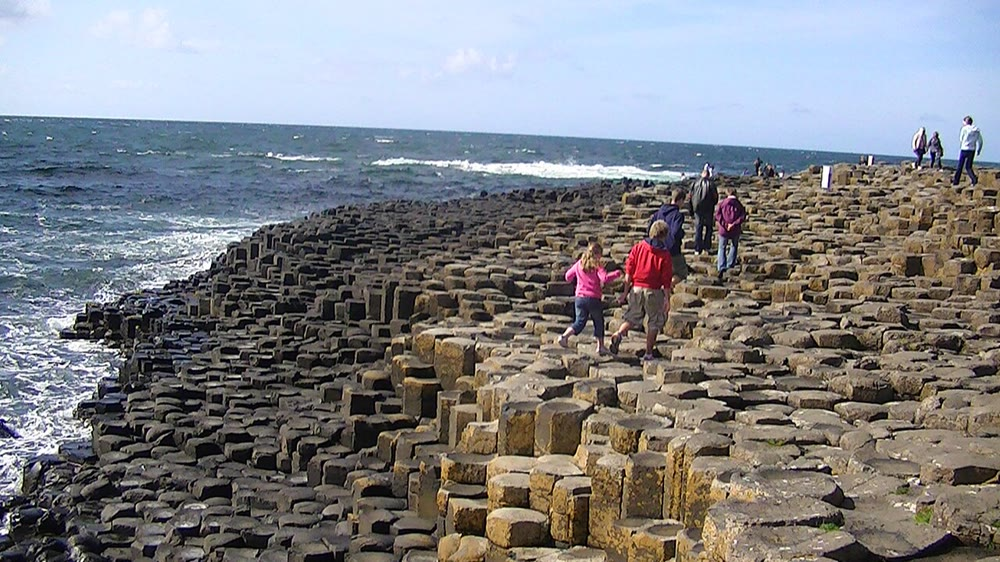
\includegraphics[height=4.3cm]{images/book2/g11-bishop-giants-causeway.jpg}\hspace{0.04\linewidth}%
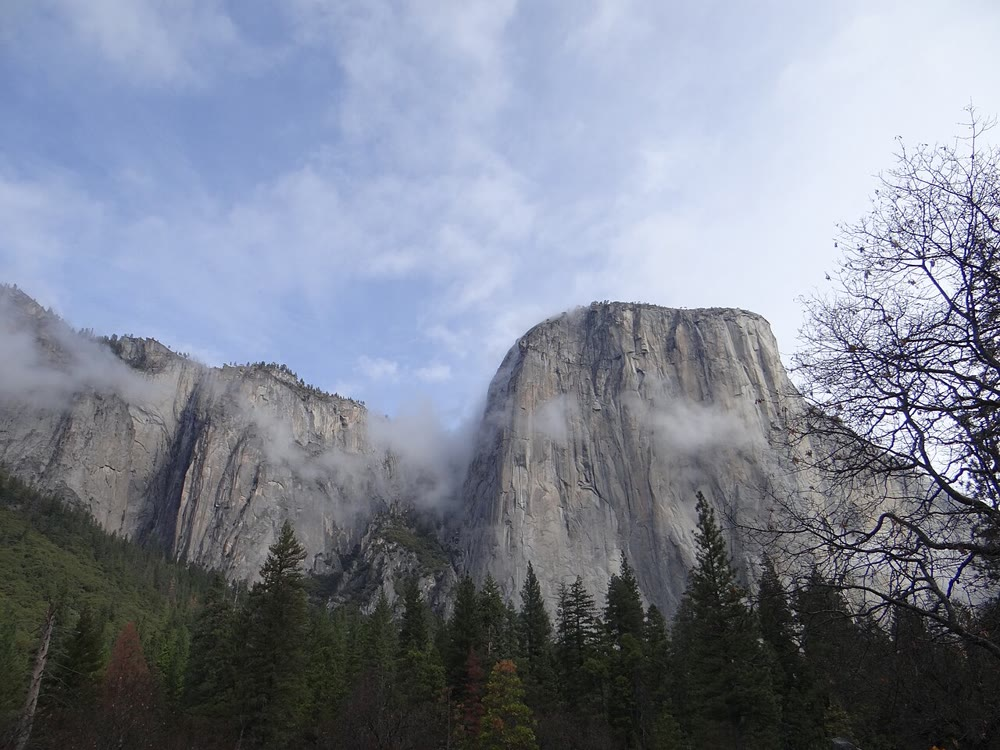
\includegraphics[height=4.3cm]{images/book2/g11-usgs-el-capitan.jpg}

{\small À esquerda: colunas de basalto da Calçada dos Gigantes, na Irlanda
do Norte. Fotografia Adam Bishop (CC~BY-SA~3.0). À direita: o El Capitan,
em Yosemite, na Califórnia, uma parede de granito de cerca de \qty{900}{m}
de altura. Fotografia U.S. Geological Survey (CC0).}
\end{omfigure}
% ledger: photo:g11-giants-causeway, photo:g11-el-capitan

\begin{recall}
O magma é rocha fundida sob a superfície; ele irrompe como lava, de modo
calmo ou explosivo (Livro 1, 7º ano). Uma rocha ígnea é uma rocha formada
quando rocha fundida esfria e se torna sólida (Livro 1, 6º ano). O basalto é uma \omterm{def:g11:igneous-rocks:volcanic-plutonic}{rocha vulcânica} escura, o granito
uma rocha clara feita de feldspato, quartzo e mica (Livro 1, 6º ano). O
\omterm{def:g11:ocean-ridges:peridotite}{peridotito} do manto funde em parte ao subir sob uma dorsal, dando o basalto e
o \omterm{def:g11:ocean-ridges:gabbro}{gabro} da \omterm{def:g11:ocean-ridges:oceanic-lithosphere}{crosta oceânica} (\cref{ch:g11:ocean-ridges}). Os \omterm{def:g11:minerals:rock-forming}{silicatos
formadores de rochas} são a olivina, os piroxênios, os anfibólios, as micas,
os feldspatos e o quartzo; os feldspatos são o feldspato potássico e o
plagioclásio, uma série que vai do rico em cálcio ao rico em sódio
(\cref{ch:g11:minerals}). O calor se espalha por condução por uma distância
de cerca de $\sqrt{\kappa t}$ num tempo $t$, onde
$\kappa$ é a difusividade térmica (\cref{ch:g11:subduction-zones}).
\end{recall}
% ledger: tulane:ridge-rocks, england:kelvin

\section{Rochas vulcânicas e rochas plutônicas}

\begin{definition}[Rocha vulcânica; rocha plutônica]\label{def:g11:igneous-rocks:volcanic-plutonic}
Uma rocha ígnea, formada pela cristalização de um magma, é
\emph{vulcânica}\index{rocha vulcanica@rocha vulcânica}
(ou extrusiva) quando o magma se solidificou na superfície da Terra, como
lava, e \emph{plutônica}\index{rocha plutonica@rocha plutônica} (ou intrusiva) quando cristalizou
em profundidade, dentro de outras rochas.
\end{definition}
% ledger: tulane:magma-types

A diferença aparece no tamanho dos cristais. Um cristal cresce acrescentando
átomos tirados do líquido em volta dele, e isso leva tempo. Na superfície,
uma lava perde o seu calor para o ar ou para a água depressa: o material
lançado no ar ou na água esfria em segundos, um derrame de lava em dias ou
semanas. No fundo, as rochas em volta são quentes e o magma perde o seu
calor devagar: uma \omterm{def:g11:igneous-rocks:intrusion}{intrusão} rasa esfria em meses ou anos, uma grande e
profunda pode levar milhões de anos. O resfriamento rápido dá muitos
cristais pequenos, ou nenhum; o resfriamento lento dá menos cristais,
muito maiores.
% ledger: tulane:cooling-times, tulane:textures

\begin{definition}[Textura]\label{def:g11:igneous-rocks:texture}
A \emph{textura}\index{textura (de uma rocha)} de uma rocha é o tamanho, a
forma e o arranjo dos seus grãos. Uma rocha ígnea é \emph{vítrea} quando não
tem cristais, \emph{de grão fino} quando os seus cristais são pequenos demais
para serem distinguidos a olho nu, e \emph{de grão grosso} quando todos
podem ser vistos.
\end{definition}
% ledger: tulane:textures

Uma lava resfriada bruscamente antes que qualquer cristal possa crescer se
torna um vidro: a obsidiana, preta e vítrea, se quebra com a \omterm{def:g11:minerals:cleavage}{fratura}
conchoidal de uma garrafa. O basalto é de grão fino: na mão, os seus
minerais não podem ser identificados, e mesmo em \omterm{def:g11:minerals:thin-section}{lâmina delgada} os cristais
são pequenos (o basalto do \cref{ch:g11:minerals}). O granito, o \omterm{def:g11:ocean-ridges:gabbro}{gabro} e o
\omterm{def:g11:igneous-rocks:rock-names}{diorito} são de grão grosso: todos os grãos aparecem.
% ledger: photo:g11-obsidian, photo:g11-basalt, tulane:textures

\begin{definition}[Fenocristal; porfirítica]\label{def:g11:igneous-rocks:porphyritic}
Um \emph{fenocristal}\index{fenocristal} é um cristal grande inserido numa
massa de cristais muito menores ou de vidro, a \emph{matriz}. Uma rocha com
fenocristais é \emph{porfirítica}\index{porfiritica@porfirítica}.
\end{definition}
% ledger: tulane:textures

Uma \omterm{def:g11:igneous-rocks:texture}{textura} \omterm{def:g11:igneous-rocks:porphyritic}{porfirítica} registra duas etapas de resfriamento: primeiro lenta,
em profundidade, enquanto os \omterm{def:g11:igneous-rocks:porphyritic}{fenocristais} cresciam num magma ainda quase todo
líquido; depois rápida, quando o magma subiu e irrompeu, ou foi injetado em
rocha fria, e o resto do líquido congelou formando a matriz.
% ledger: tulane:textures

\begin{omfigure}
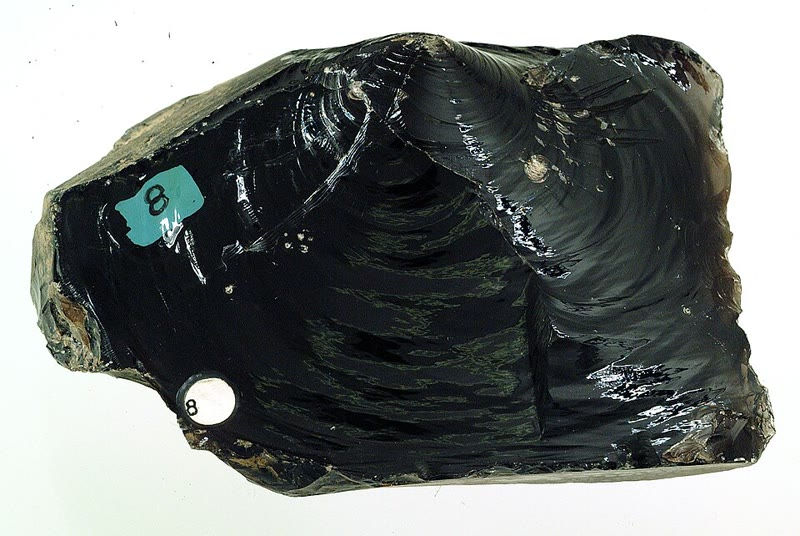
\includegraphics[height=2.75cm]{images/book2/g11-geodil-obsidian.jpg}\hfill
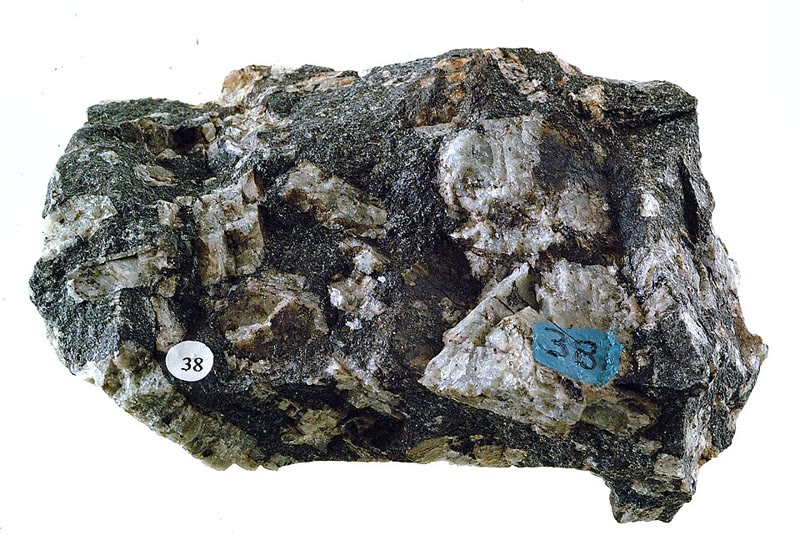
\includegraphics[height=2.75cm]{images/book2/g11-geodil-diabase-porphyry.jpg}\hfill
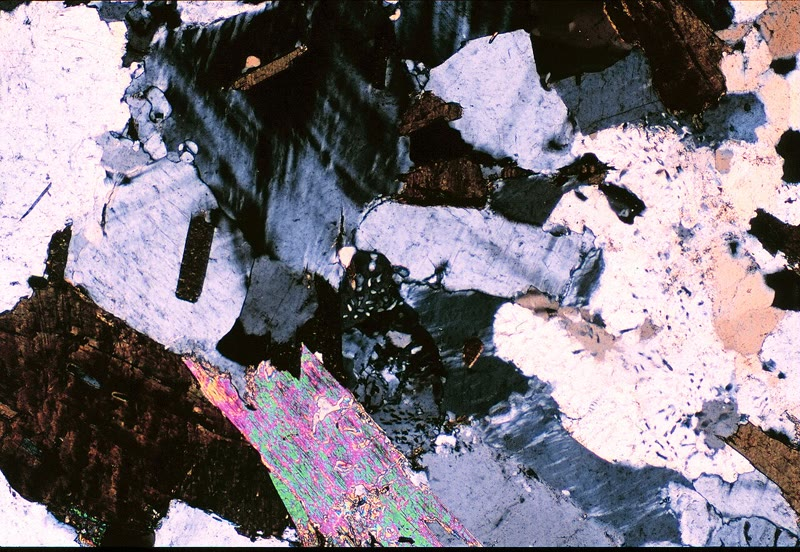
\includegraphics[height=2.75cm]{images/book2/g11-geodil-granite-xpl.jpg}\hfill
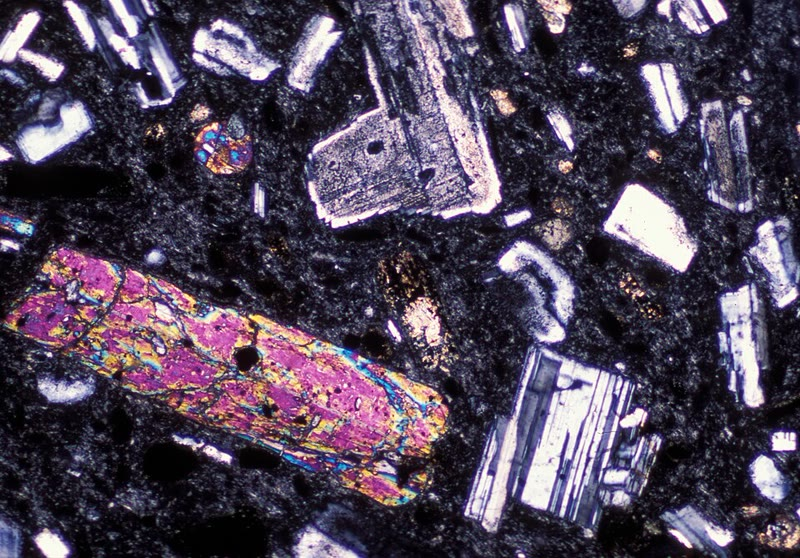
\includegraphics[height=2.75cm]{images/book2/g11-geodil-andesite-xpl.jpg}

{\small Da esquerda para a direita: obsidiana, um vidro vulcânico, com a sua
\omterm{def:g11:minerals:cleavage}{fratura} conchoidal curva (\qty{9.5}{cm} de largura); uma rocha \omterm{def:g11:igneous-rocks:porphyritic}{porfirítica},
\omterm{def:g11:igneous-rocks:porphyritic}{fenocristais} de plagioclásio em blocos numa matriz mais fina (\qty{9}{cm});
depois duas \omterm{def:g11:minerals:thin-section}{lâminas delgadas} entre polarizadores cruzados: um granito, com
todos os grãos grandes e encaixados --- biotita marrom, uma muscovita de
cores vivas, plagioclásio listrado, quartzo cinza e branco; um \omterm{def:g11:igneous-rocks:rock-names}{andesito},
\omterm{def:g11:igneous-rocks:porphyritic}{fenocristais} de plagioclásio e de anfibólio numa matriz de grão fino.
Fotografias Twyla Baker, Mike Davis e Darla Sondrol, Geology Digital Image
Library (CC0).}
\end{omfigure}
% ledger: photo:g11-obsidian, photo:g11-diabase-porphyry, photo:g11-granite-xpl, photo:g11-andesite-xpl

\section{Dar nome às rochas ígneas}

A segunda chave de uma rocha ígnea é a sua química, e acima de tudo o seu
teor de sílica, \ce{SiO2}, que nos magmas comuns vai de cerca de
\qty{45}{\percent} a cerca de \qty{75}{\percent} da massa.

\begin{definition}[Máfico; intermediário; félsico]\label{def:g11:igneous-rocks:felsic-mafic}
Um magma, ou a rocha que ele forma, é \emph{máfico}\index{mafico@máfico}
quando contém cerca de \qty{45}{\percent} a \qty{55}{\percent} de \ce{SiO2} e
é rico em ferro, magnésio e cálcio; \emph{intermediário}\index{intermediaria (rocha)@intermediária (rocha)}
entre \qty{55}{\percent} e \qty{65}{\percent}; \emph{félsico}\index{felsico@félsico}
quando contém cerca de \qty{65}{\percent} a \qty{75}{\percent} de \ce{SiO2} e
é pobre em ferro, magnésio e cálcio, mas rico em sódio e potássio.
\end{definition}
% ledger: tulane:magma-types, earle:magma-oxides

Cada tipo de magma dá duas rochas, uma \omterm{def:g11:igneous-rocks:volcanic-plutonic}{vulcânica} e de grão fino, outra
\omterm{def:g11:igneous-rocks:volcanic-plutonic}{plutônica} e de grão grosso, com a mesma química. O basalto e o \omterm{def:g11:ocean-ridges:gabbro}{gabro} são o
par \omterm{def:g11:igneous-rocks:felsic-mafic}{máfico}, visto com a \omterm{def:g11:ocean-ridges:oceanic-lithosphere}{crosta oceânica}; o granito é a \omterm{def:g11:igneous-rocks:volcanic-plutonic}{rocha plutônica}
\omterm{def:g11:igneous-rocks:felsic-mafic}{félsica}. Três nomes completam o conjunto.

\begin{definition}[Andesito; diorito; riolito]\label{def:g11:igneous-rocks:rock-names}
O \emph{andesito}\index{andesito} e o \emph{diorito}\index{diorito} são a
\omterm{def:g11:igneous-rocks:volcanic-plutonic}{rocha vulcânica} e a \omterm{def:g11:igneous-rocks:volcanic-plutonic}{rocha plutônica} de composição \omterm{def:g11:igneous-rocks:felsic-mafic}{intermediária}, feitas
principalmente de plagioclásio com anfibólio ou piroxênio. O
\emph{riolito}\index{riolito} é a \omterm{def:g11:igneous-rocks:volcanic-plutonic}{rocha vulcânica} de composição \omterm{def:g11:igneous-rocks:felsic-mafic}{félsica}, o
equivalente de grão fino do granito.
\end{definition}
% ledger: tulane:magma-types, earle:bowen, photo:g11-andesite, photo:g11-diorite

\begin{omfigure}
\begin{tikzpicture}[font=\footnotesize, x=0.4cm]
  % columns: SiO2 45 to 75 % mapped to x = 45 to 75 (0.4 cm per %)
  \begin{scope}[xshift=-18cm]
  \fill[omLithBasalt!45] (45,0) rectangle (55,2.4);
  \fill[omLithBasalt!20] (55,0) rectangle (65,2.4);
  \fill[omLithGranite!45] (65,0) rectangle (75,2.4);
  \draw[black!60] (45,0) rectangle (75,2.4);
  \draw[black!60] (55,0) -- (55,2.4); \draw[black!60] (65,0) -- (65,2.4);
  \draw[black!60] (45,1.2) -- (75,1.2);
  \foreach \x/\a/\b in {50/basalto/gabro, 60/andesito/diorito, 70/riolito/granito}{
    \node[font=\small\bfseries, text height=1.6ex, text depth=0.3ex] at (\x,1.8) {\a};
    \node[font=\small\bfseries, text height=1.6ex, text depth=0.3ex] at (\x,0.6) {\b};}
  \node[anchor=east, align=right] at (44.4,1.8) {grão fino\\(vulcânica)};
  \node[anchor=east, align=right] at (44.4,0.6) {grão grosso\\(plutônica)};
  \node[anchor=south] at (50,2.45) {máfica};
  \node[anchor=south] at (60,2.45) {intermediária};
  \node[anchor=south] at (70,2.45) {félsica};
  % minerals (a drawing: where each mineral is common)
  \foreach \y/\a/\b/\m/\c in {-0.55/45.2/52/olivina/omLithBasalt!80!black,
      -1.15/45.2/61/piroxênio/omLithBasalt!65!black,
      -1.75/52/69/anfibólio/black!60,
      -2.35/57/74.8/biotita/black!75,
      -2.95/45.2/72/plagioclásio/omDef!45,
      -3.55/63/74.8/feldspato potássico/omLithGranite!90!red,
      -4.15/64/74.8/quartzo/black!20,
      -4.75/68/74.8/muscovita/black!35}{
    \fill[\c] (\a,\y) .. controls ({\a+1.2},{\y+0.22}) and ({\b-1.2},{\y+0.22}) .. (\b,\y)
              .. controls ({\b-1.2},{\y-0.22}) and ({\a+1.2},{\y-0.22}) .. (\a,\y) -- cycle;
    \node[anchor=east] at (44.4,\y) {\m};}
  \node[font=\scriptsize, text=black!75] at (50,-2.95) {rico em cálcio};
  \node[font=\scriptsize, text=omDef!80!black, anchor=west] at (72.3,-2.95) {rico em sódio};
  % SiO2 axis
  \draw[-{Stealth[length=4pt]}] (45,-5.35) -- (75.8,-5.35);
  \foreach \x in {45,50,...,75} {\draw (\x,-5.35) -- (\x,-5.45); \node[anchor=north] at (\x,-5.45) {\x};}
  \node[anchor=north] at (60,-5.85) {\ce{SiO2} (\unit{\percent} da massa)};
  \draw[black!30, dashed] (55,0) -- (55,-5.35); \draw[black!30, dashed] (65,0) -- (65,-5.35);
  \end{scope}
\end{tikzpicture}

{\small Dar nome às rochas ígneas comuns (um desenho). Colunas: o teor de
sílica do magma; linhas: rochas de grão fino (\omterm{def:g11:igneous-rocks:volcanic-plutonic}{vulcânicas}) e de grão grosso
(\omterm{def:g11:igneous-rocks:volcanic-plutonic}{plutônicas}). Embaixo, onde cada mineral formador de rochas é comum: olivina
e piroxênio nas rochas \omterm{def:g11:igneous-rocks:felsic-mafic}{máficas}, com plagioclásio rico em cálcio; anfibólio e
plagioclásio nas rochas \omterm{def:g11:igneous-rocks:felsic-mafic}{intermediárias}; feldspato potássico, quartzo,
plagioclásio rico em sódio e micas nas rochas \omterm{def:g11:igneous-rocks:felsic-mafic}{félsicas}. Os limites são
graduais.}
\end{omfigure}
% ledger: tulane:magma-types, earle:bowen, earle:magma-oxides, photo:g11-andesite, photo:g11-diorite, photo:g11-granite, nps:granite-minerals

\begin{method}[Dar nome a uma rocha ígnea]\label{met:g11:igneous-rocks:naming}
\begin{enumerate}
  \item Observe a \omterm{def:g11:igneous-rocks:texture}{textura}: vítrea, de grão fino ou de grão grosso;
        \omterm{def:g11:igneous-rocks:porphyritic}{porfirítica} ou não. Grão fino ou vítrea indica \omterm{def:g11:igneous-rocks:volcanic-plutonic}{vulcânica} (ou uma
        \omterm{def:g11:igneous-rocks:intrusion}{intrusão} pequena, resfriada depressa); grão grosso indica \omterm{def:g11:igneous-rocks:volcanic-plutonic}{plutônica}.
  \item Identifique os minerais que podem ser vistos
        (\cref{met:g11:minerals:identify}): o quartzo e o feldspato potássico
        apontam para \omterm{def:g11:igneous-rocks:felsic-mafic}{félsica}, o anfibólio com plagioclásio para \omterm{def:g11:igneous-rocks:felsic-mafic}{intermediária},
        a olivina e o piroxênio para \omterm{def:g11:igneous-rocks:felsic-mafic}{máfica}. Numa rocha de grão fino, use os
        \omterm{def:g11:igneous-rocks:porphyritic}{fenocristais}, a cor da matriz --- escura para \omterm{def:g11:igneous-rocks:felsic-mafic}{máfica}, clara para
        \omterm{def:g11:igneous-rocks:felsic-mafic}{félsica} --- como indício, ou uma análise química.
  \item Leia o nome no cruzamento da linha e da coluna do quadro.
\end{enumerate}
\end{method}

\begin{example}[Dois basaltos]
Uma rocha escura de um derrame de lava é de grão fino em toda a sua massa;
outra, do mesmo vulcão, mostra grãos verdes de olivina de alguns milímetros
numa matriz escura. As duas são \omterm{def:g11:igneous-rocks:felsic-mafic}{máficas} e de grão fino: as duas são
basaltos. A segunda é um basalto \omterm{def:g11:igneous-rocks:porphyritic}{porfirítico}: a sua olivina cresceu primeiro,
lentamente, no magma sob o vulcão, antes que a lava irrompesse e congelasse
em volta dela.
\end{example}
% ledger: photo:g11-olivine, earle:bowen, tulane:textures

\begin{omfigure}
\makebox[0.32\linewidth]{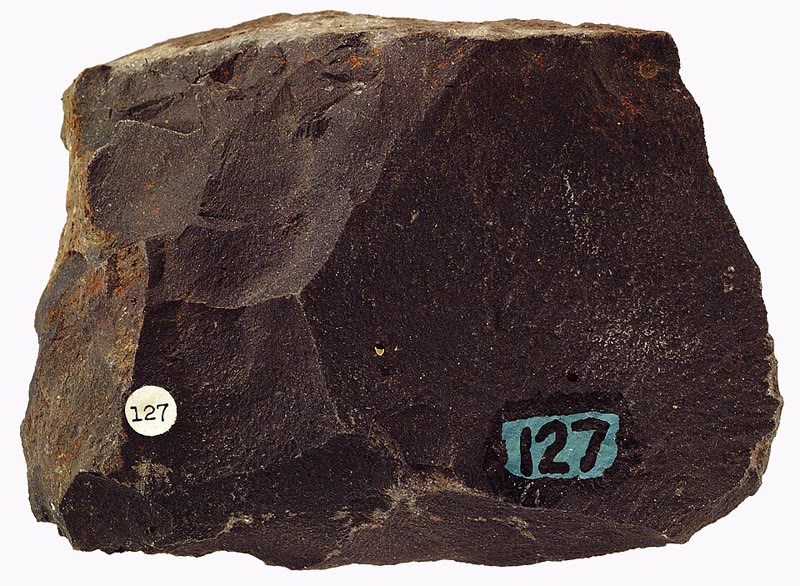
\includegraphics[height=2.9cm]{images/book2/g11-geodil-basalt.jpg}}\hfill
\makebox[0.32\linewidth]{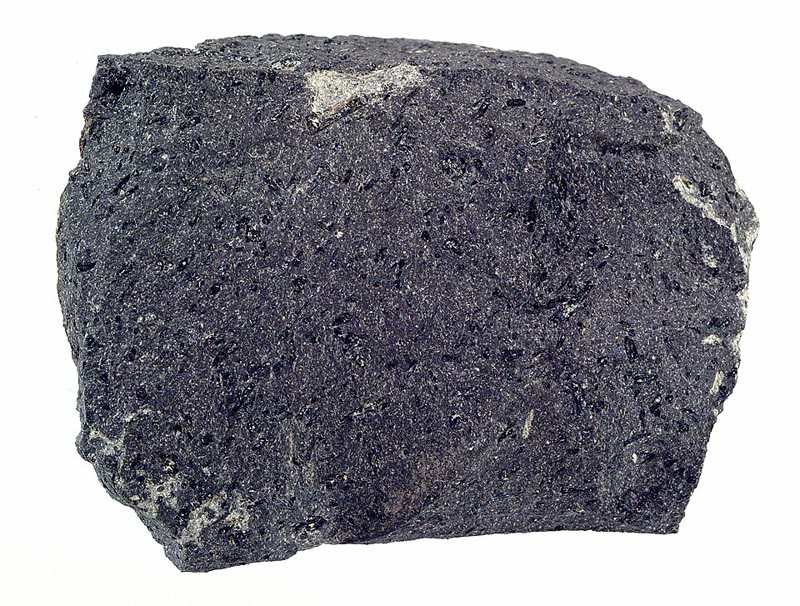
\includegraphics[height=2.9cm]{images/book2/g11-geodil-andesite.jpg}}\hfill
\makebox[0.32\linewidth]{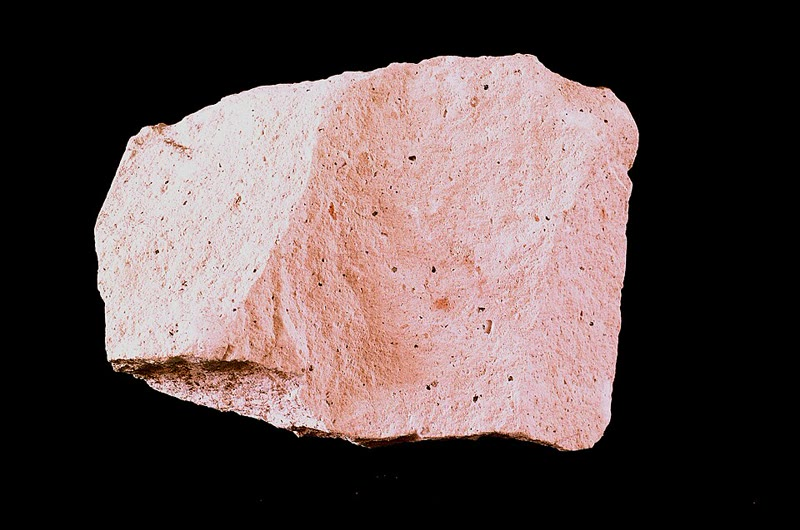
\includegraphics[height=2.9cm]{images/book2/g11-geodil-rhyolite.jpg}}

\smallskip
\makebox[0.32\linewidth]{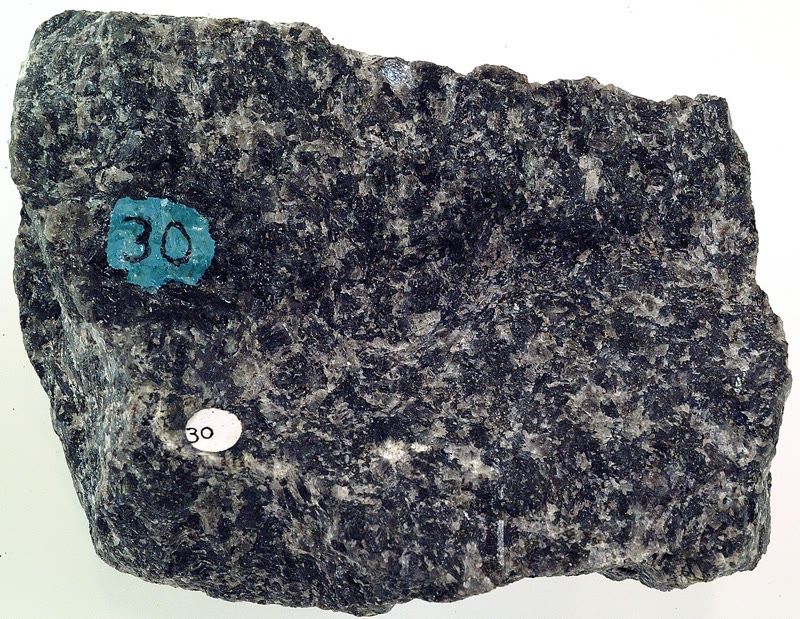
\includegraphics[height=2.9cm]{images/book2/g11-geodil-gabbro.jpg}}\hfill
\makebox[0.32\linewidth]{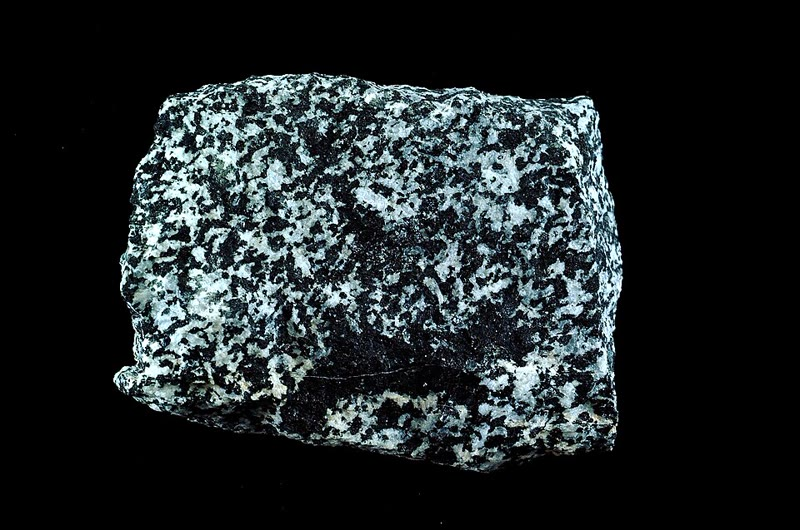
\includegraphics[height=2.9cm]{images/book2/g11-geodil-diorite.jpg}}\hfill
\makebox[0.32\linewidth]{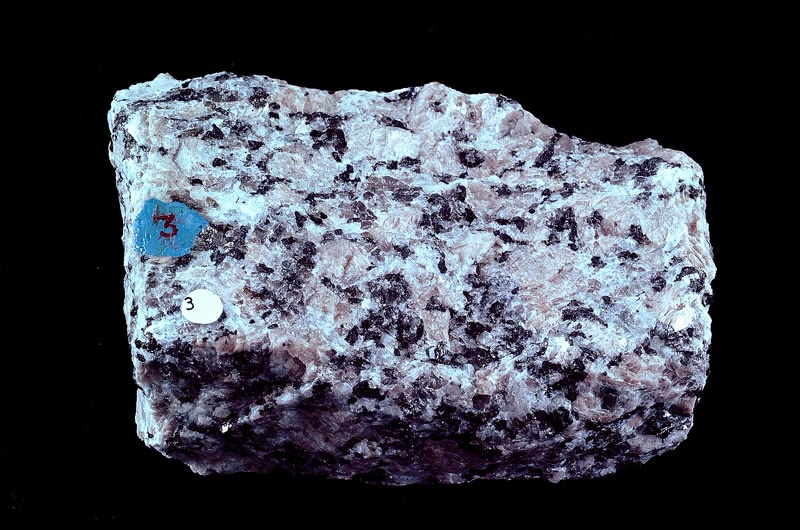
\includegraphics[height=2.9cm]{images/book2/g11-geodil-granite.jpg}}

{\small Os três pares de rochas ígneas, de \omterm{def:g11:igneous-rocks:felsic-mafic}{máfica} a \omterm{def:g11:igneous-rocks:felsic-mafic}{félsica}, da esquerda
para a direita: \omterm{def:g11:igneous-rocks:volcanic-plutonic}{vulcânicas} em cima, \omterm{def:g11:igneous-rocks:volcanic-plutonic}{plutônicas} embaixo. Em cima: um basalto
de grão fino; um \omterm{def:g11:igneous-rocks:rock-names}{andesito}, pequenos cristais de anfibólio numa matriz de
grão fino (cerca de \qty{10}{cm}); um \omterm{def:g11:igneous-rocks:rock-names}{riolito} rosa. Embaixo: \omterm{def:g11:ocean-ridges:gabbro}{gabro}
(\qty{9}{cm}); \omterm{def:g11:igneous-rocks:rock-names}{diorito}, hornblenda preta e plagioclásio vítreo
(\qty{10}{cm}); um granito grosso com grandes feldspatos potássicos
rosa-claros, plagioclásio cinza, quartzo, biotita e hornblenda
(\qty{10}{cm}). Fotografias Nessa Eull, Twyla Baker, Joseph H.~Hartman,
Darla Sondrol e Dexter Perkins, Geology Digital Image Library (CC0).}
\end{omfigure}
% ledger: photo:g11-basalt, photo:g11-andesite, photo:g11-rhyolite, photo:g11-gabbro, photo:g11-diorite, photo:g11-granite

\section{A ordem de cristalização}

Um magma não congela a uma única temperatura, como a água. Os seus minerais
aparecem um depois do outro à medida que ele esfria, cada um na sua própria
faixa de temperatura, de modo que um magma que esfria pode conter cristais e
ainda ser quase todo líquido.

\begin{history}[Os experimentos de Bowen]
Norman L.~Bowen (1887--1956) entrou no Laboratório de Geofísica da
Instituição Carnegie, em Washington, em 1912. Trabalhando sobretudo com
magmas basálticos, ele fundia uma rocha num forno, deixava-a esfriar
lentamente até uma temperatura escolhida, de modo que alguns minerais se
formassem, e então a resfriava bruscamente, tão depressa que o líquido
restante se tornava um vidro. Ao microscópio, os cristais mostravam que
minerais tinham se formado acima daquela temperatura. Repetido a
temperaturas cada vez mais baixas, o experimento dava a ordem em que os
minerais aparecem. Bowen publicou essa ordem como uma série de reação em
1922, e o seu livro \emph{The Evolution of the Igneous Rocks} em 1928.
\end{history}
% ledger: carnegie:bowen, earle:bowen

\begin{omfigure}
\begin{tikzpicture}[font=\footnotesize, box/.style={draw=black!60, rounded corners=2pt, fill=#1, minimum width=3.0cm, minimum height=0.62cm, align=center}]
  \node[box=omLithBasalt!45] (ol) at (0,0) {olivina};
  \node[box=omLithBasalt!35] (px) at (0,-1.1) {piroxênio};
  \node[box=black!15] (am) at (0,-2.2) {anfibólio};
  \node[box=black!25] (bi) at (0,-3.3) {biotita};
  \draw[-{Stealth[length=4pt]}, line width=0.8pt] (ol) -- (px);
  \draw[-{Stealth[length=4pt]}, line width=0.8pt] (px) -- (am);
  \draw[-{Stealth[length=4pt]}, line width=0.8pt] (am) -- (bi);
  \node[align=center, anchor=south] at (0,0.45) {\textbf{ramo descontínuo}\\cada mineral reage com o líquido\\e se transforma no seguinte};
  % continuous branch: a wedge from Ca-rich to Na-rich
  \fill[left color=omDef!55, right color=omDef!12, shading angle=180] (5.0,-0.9) -- (6.6,-0.9) -- (6.6,-3.5) -- (5.0,-3.5) -- cycle;
  \shade[top color=omDef!60, bottom color=omDef!10, draw=black!60, rounded corners=2pt] (4.3,-0.85) rectangle (7.3,-3.55);
  \node[align=center] at (5.8,-1.3) {plagioclásio\\rico em cálcio};
  \node[align=center] at (5.8,-3.15) {plagioclásio\\rico em sódio};
  \draw[-{Stealth[length=4pt]}, line width=0.8pt] (5.8,-1.65) -- (5.8,-2.7);
  \node[align=center, anchor=south] at (5.8,0.45) {\textbf{ramo contínuo}\\o plagioclásio muda\\gradualmente};
  % last minerals
  \node[box=omLithGranite!45, minimum width=7.6cm] (last) at (2.9,-4.75) {feldspato potássico, quartzo, (muscovita)};
  \draw[-{Stealth[length=4pt]}, line width=0.8pt] (bi) -- (bi |- last.north);
  \draw[-{Stealth[length=4pt]}, line width=0.8pt] (5.8,-3.55) -- (5.8,-4.43);
  % temperature arrow
  \draw[-{Stealth[length=5pt]}, line width=1pt, omThm] (-2.6,0.3) -- (-2.6,-4.9);
  \node[anchor=east, align=right, text=omThm] at (-2.75,0.1) {primeiro,\\\qtyrange{1200}{1300}{\degreeCelsius}};
  \node[anchor=east, align=right, text=omThm] at (-2.75,-4.7) {por último, cerca de\\\qtyrange{750}{800}{\degreeCelsius}};
  \node[anchor=east, align=right, text=omThm] at (-2.75,-2.3) {temperatura\\em queda};
\end{tikzpicture}

{\small A ordem em que os minerais cristalizam a partir de um magma que
esfria (a série de reação de Bowen, um desenho). A olivina se forma
primeiro; o plagioclásio começa mais ou menos onde começa o piroxênio, rico
em cálcio no início, depois cada vez mais rico em sódio. O feldspato
potássico, o quartzo e às vezes a muscovita se formam por último, a partir
do que resta de um líquido rico em sílica.}
\end{omfigure}
% ledger: earle:bowen

A palavra \emph{reação} importa. A olivina só é estável a alta temperatura:
à medida que o magma esfria, os cristais de olivina reagem com a sílica do
líquido e se transformam em piroxênio,
\[
  \ce{Mg2SiO4 + SiO2 -> 2 MgSiO3},
\]
e assim por diante ao longo do ramo, enquanto houver sílica no líquido. Ao
longo do outro ramo, os cristais de plagioclásio continuam crescendo, mas
cada nova camada é mais rica em sódio que a anterior: um cristal de
plagioclásio pode ser zonado, de um núcleo rico em cálcio a uma borda rica
em sódio, como os \omterm{def:g11:igneous-rocks:porphyritic}{fenocristais} de plagioclásio do \omterm{def:g11:igneous-rocks:rock-names}{andesito} acima.
% ledger: earle:bowen, photo:g11-andesite-xpl

A série explica o quadro. Um magma \omterm{def:g11:igneous-rocks:felsic-mafic}{máfico} esgota a sua sílica cedo: ele
cristaliza olivina, piroxênio e plagioclásio rico em cálcio, e dá um \omterm{def:g11:ocean-ridges:gabbro}{gabro}
se esfria devagar no subsolo, um basalto se esfria depressa na superfície.
Só um magma rico em sílica chega ao fim da série e forma feldspato potássico
e quartzo: os minerais do granito e do \omterm{def:g11:igneous-rocks:rock-names}{riolito}. Como um magma muda de
composição no caminho, quando os seus primeiros cristais são separados do
líquido, é assunto do segundo ano da universidade.
% ledger: earle:bowen, tulane:bowen

\section{As intrusões}

O magma sobe porque é menos denso que as rochas em volta, abrindo caminho
pelas fraturas e alargando-as. Grande parte dele nunca chega à superfície:
ele cristaliza na crosta em \omterm{def:g11:igneous-rocks:intrusion}{intrusões}, que só são vistas depois que a erosão
retirou as rochas de cima.
% ledger: tulane:intrusions

\begin{definition}[Dique; soleira; plúton]\label{def:g11:igneous-rocks:intrusion}
Uma \emph{intrusão}\index{intrusao@intrusão} é um corpo de rocha ígnea que
cristalizou dentro de outras rochas. Um \emph{dique}\index{dique} é uma
lâmina de rocha ígnea que corta as camadas ou as estruturas das rochas em
que penetra; uma \emph{soleira}\index{soleira} é uma lâmina paralela às
camadas, entre elas. Um \emph{plúton}\index{pluton@plúton} é uma grande
intrusão de qualquer forma, formada em profundidade; muitos plútons reunidos
formam um batólito (\cref{ch:g12:subduction-magmatism}).
\end{definition}
% ledger: tulane:intrusions

Os \omterm{def:g11:igneous-rocks:intrusion}{diques} têm em geral menos de \qty{20}{m} de largura, e as \omterm{def:g11:igneous-rocks:intrusion}{soleiras} menos
de \qty{50}{m} de espessura; uma \omterm{def:g11:igneous-rocks:intrusion}{soleira} costuma ser alimentada por um
\omterm{def:g11:igneous-rocks:intrusion}{dique}. Os \omterm{def:g11:igneous-rocks:intrusion}{diques} e as \omterm{def:g11:igneous-rocks:intrusion}{soleiras} rasos esfriam depressa: eles são de grão
fino, às vezes \omterm{def:g11:igneous-rocks:porphyritic}{porfiríticos}. Contra a rocha fria em que penetram, as suas
bordas esfriam mais depressa ainda e têm grão ainda mais fino que o centro:
uma \emph{margem resfriada}, a marca de um corpo que estava quente quando se
instalou. A Sierra Nevada da Califórnia, onde fica Yosemite, é um batólito:
as rochas graníticas cuja densidade foi medida no \cref{ch:g11:minerals} vêm
de cerca de duzentos dos seus \omterm{def:g11:igneous-rocks:intrusion}{plútons}.
% ledger: tulane:intrusions, usgs91:sierra, photo:g11-el-capitan

\begin{omfigure}
\begin{tikzpicture}[font=\footnotesize, scale=0.9]
  % layered host rocks
  \fill[omLithSand] (0,0) rectangle (14,-1.0);
  \fill[omLithShale] (0,-1.0) rectangle (14,-2.0);
  \fill[omLithLime] (0,-2.0) rectangle (14,-3.0);
  \fill[omLithSand] (0,-3.0) rectangle (14,-4.0);
  \fill[omLithShale] (0,-4.0) rectangle (14,-6.4);
  \foreach \y in {-1,-2,-3,-4} \draw[black!35] (0,\y) -- (14,\y);
  % pluton
  \fill[omLithGranite, draw=black!60] (2.2,-6.4) .. controls (2.4,-4.6) and (3.6,-4.1) .. (5.5,-4.15)
     .. controls (7.4,-4.2) and (9.0,-4.5) .. (9.6,-6.4) -- cycle;
  % sill between the limestone and the shale, fed by the dyke
  \fill[omLithBasalt, draw=black!60] (7.3,-1.88) -- (12.6,-1.88) .. controls (12.9,-1.9) and (12.9,-2.1) .. (12.6,-2.12) -- (7.3,-2.12) -- cycle;
  % dyke from the pluton to the volcano
  \fill[omLithBasalt, draw=black!60] (7.0,-4.18) -- (7.3,-4.2) -- (7.3,0) -- (7.0,0) -- cycle;
  % a second dyke cutting across the layers, not reaching the surface
  \fill[omLithBasalt, draw=black!60] (3.9,-4.15) -- (4.15,-4.15) -- (2.95,-0.6) -- (2.75,-0.6) -- cycle;
  % volcano and lava flow
  \fill[black!65] (5.75,0) -- (7.15,1.35) -- (8.55,0) -- cycle;
  \fill[omLithBasalt!80!black] (8.4,0) -- (11.6,0) -- (11.6,0.1) .. controls (10.5,0.16) and (9.2,0.22) .. (8.3,0.15) -- cycle;
  \draw[black!70] (0,0) -- (5.75,0); \draw[black!70] (8.55,0) -- (14,0);
  % labels
  \node[anchor=south] at (7.15,1.4) {vulcão};
  \draw[black!60] (10.5,0.15) -- (11.2,0.8); \node[anchor=south west, inner sep=1pt] at (11.2,0.8) {derrame de lava};
  \draw[black!60] (7.3,-0.5) -- (8.3,-0.5); \node[anchor=west, fill=omLithSand, inner sep=1pt] at (8.3,-0.5) {dique (corta as camadas)};
  \draw[black!60] (11.0,-2.0) -- (11.0,-2.55); \node[anchor=north, fill=omLithLime, inner sep=1pt] at (11.0,-2.55) {soleira (entre as camadas)};
  \draw[black!60] (3.4,-2.5) -- (1.9,-2.5); \node[anchor=east, fill=omLithLime, inner sep=1pt] at (1.9,-2.5) {dique};
  \node[align=center] at (5.9,-5.5) {plúton};
  \node[anchor=east, fill=omLithShale, inner sep=1pt] at (13.85,-5.3) {rochas sedimentares em camadas};
\end{tikzpicture}

{\small \omterm{def:g11:igneous-rocks:intrusion}{Intrusões} (um desenho, fora de escala). Um \omterm{def:g11:igneous-rocks:intrusion}{plúton} cristaliza em
profundidade; \omterm{def:g11:igneous-rocks:intrusion}{diques} cortam as camadas das rochas acima dele, um deles
alimentando um vulcão; uma \omterm{def:g11:igneous-rocks:intrusion}{soleira} se espalha entre duas camadas. Só a
erosão das rochas de cima deixa esses corpos expostos na superfície.}
\end{omfigure}
% ledger: tulane:intrusions

Quanto tempo uma \omterm{def:g11:igneous-rocks:intrusion}{intrusão} leva para cristalizar? Considere uma lâmina de
magma --- um \omterm{def:g11:igneous-rocks:intrusion}{dique} ou uma \omterm{def:g11:igneous-rocks:intrusion}{soleira} --- de espessura $b$, que perde o seu calor
por condução para a rocha dos dois lados. As únicas grandezas que ditam o
ritmo são a espessura $b$, em metros, e a difusividade térmica $\kappa$, em
\unit{m^2/s}; o único tempo que se pode construir com elas é $b^2/\kappa$.
% ledger: england:kelvin, delaney86:example

\begin{proposition}[O tempo de resfriamento de uma lâmina de magma]\label{prop:g11:igneous-rocks:cooling}
Uma lâmina de magma de espessura $b$ que esfria por condução se solidifica
num tempo
\[
  t = C\,\frac{b^2}{\kappa},
\]
onde $\kappa$ é a difusividade térmica das rochas e $C$ um número fixado
pelas temperaturas do magma e da rocha em volta e pelo calor liberado
quando o magma cristaliza. Dobrar a espessura multiplica o tempo por quatro.
(Admitido; o valor de $C$ vem de um modelo calculado.)
\end{proposition}
% ledger: delaney86:properties, delaney86:example

Para um magma basáltico intrudido a \qty{1150}{\degreeCelsius} numa rocha a
\qty{50}{\degreeCelsius}, que cristaliza completamente a
\qty{950}{\degreeCelsius} e libera \qty{900}{MJ} de calor para cada metro
cúbico que cristaliza, com $\kappa = \qty{1e-6}{m^2/s}$, o modelo dá
$C \approx 0.21$. Uma lâmina de \qty{2}{m} de espessura se solidifica então
em cerca de dez dias, uma \omterm{def:g11:igneous-rocks:intrusion}{soleira} de \qty{20}{m} em cerca de dois anos e
meio, uma de \qty{100}{m} em cerca de sessenta e cinco anos. Sem o calor de
cristalização, os tempos seriam três vezes mais curtos: o magma que
cristaliza mantém a si mesmo aquecido.
% values (dyke_cooling.py): t2_day 9.55, t20_yr 2.61, t100_yr 65.3, latent_factor 2.94; C = 8.2475e7 s / 4e8 s = 0.206
% ledger: delaney86:example, delaney86:properties, england:kelvin

\begin{omfigure}
\begin{tikzpicture}
\begin{axis}[omrecord, name=times, width=0.45\linewidth, height=5.0cm, xmode=log, ymode=log,
  xmin=0.8, xmax=130, ymin=1e-3, ymax=200, xlabel={espessura da lâmina (\unit{m})},
  ylabel={tempo de solidificação (anos)},
  legend style={font=\scriptsize, at={(0.5,-0.4)}, anchor=north, legend columns=2,
    /tikz/every even column/.append style={column sep=4pt}}]
% computed in figdata/grade-11/dyke_cooling.py; ledger: delaney86:*, england:kelvin
\addplot[omThm, line width=1pt, mark=*, mark size=1.4pt] table[x=b, y=t_yr] {figdata/out/grade-11-dyke_cooling-times.dat};
\addplot[omDef, line width=1pt, dashed, mark=o, mark size=1.4pt] table[x=b, y=t0_yr] {figdata/out/grade-11-dyke_cooling-times.dat};
\legend{com calor de cristalização, sem}
\end{axis}
\begin{axis}[omrecord, at={(times.east)}, anchor=west, xshift=1.6cm, width=0.45\linewidth, height=5.0cm,
  xmin=-28, xmax=28, ymin=0, ymax=1300, xlabel={distância ao centro da soleira (\unit{m})},
  ylabel={temperatura (\unit{\degreeCelsius})},
  legend style={font=\scriptsize, at={(0.5,-0.4)}, anchor=north, legend columns=4,
    /tikz/every even column/.append style={column sep=4pt}}]
\fill[omLithBasalt!30] (axis cs:-10,0) rectangle (axis cs:10,1300);
\draw[black!50, dashed] (axis cs:-28,950) -- (axis cs:28,950);
\node[font=\scriptsize, anchor=south east, text=black!60] at (axis cs:27,955) {solidus};
\node[font=\scriptsize, anchor=north] at (axis cs:0,1290) {soleira};
% computed in figdata/grade-11/dyke_cooling.py
\addplot[omProp, line width=0.9pt] table[x=x, y=T1] {figdata/out/grade-11-dyke_cooling-profiles.dat};
\addplot[omThm, line width=0.9pt] table[x=x, y=T2] {figdata/out/grade-11-dyke_cooling-profiles.dat};
\addplot[omDef, line width=0.9pt] table[x=x, y=T3] {figdata/out/grade-11-dyke_cooling-profiles.dat};
\addplot[black, line width=0.9pt] table[x=x, y=T4] {figdata/out/grade-11-dyke_cooling-profiles.dat};
\legend{30 dias, 6 meses, 1 ano, 2 anos}
\end{axis}
\end{tikzpicture}

{\small Uma lâmina de magma basáltico que esfria por condução (modelo
calculado). À esquerda: o tempo que ela leva para se solidificar, em função
da sua espessura, em eixos logarítmicos: uma reta de inclinação 2, com o
tempo crescendo como o quadrado da espessura. À direita: as temperaturas
através de uma \omterm{def:g11:igneous-rocks:intrusion}{soleira} de \qty{20}{m} de espessura (sombreada), intrudida a
\qty{1150}{\degreeCelsius} numa rocha a \qty{50}{\degreeCelsius}. As bordas
caem abaixo do solidus de imediato, o centro só depois de cerca de dois anos
e meio.}
\end{omfigure}
% values (dyke_cooling.py): profiles at 30, 180, 365, 730 days; contact about 690 degC (Delaney: 690)

O modelo também mostra a margem resfriada se formando. A rocha no contato
salta de imediato para cerca de \qty{690}{\degreeCelsius}, muito abaixo do
solidus: os primeiros centímetros da \omterm{def:g11:igneous-rocks:intrusion}{soleira} congelam em menos de um dia,
enquanto o seu centro continua líquido por anos. As \omterm{def:g11:igneous-rocks:intrusion}{intrusões} reais são mais
complicadas --- as propriedades das rochas mudam com a temperatura, a água
circula, um \omterm{def:g11:igneous-rocks:intrusion}{plúton} profundo fica numa rocha que já está quente e pode ser
realimentado várias vezes ---, e é por isso que as grandes \omterm{def:g11:igneous-rocks:intrusion}{intrusões}
profundas levam muito mais tempo para esfriar do que a lei, com uma rocha
encaixante fria, sugeriria.
% ledger: delaney86:example, tulane:cooling-times
% values (dyke_cooling.py): margin_day_20m 0.58 (cell 12.5 cm from the contact)

\section{Exercícios}

\begin{exercise}[$\star$]\label{exo:g11:igneous-rocks:1}
Defina uma \omterm{def:g11:igneous-rocks:volcanic-plutonic}{rocha vulcânica} e uma \omterm{def:g11:igneous-rocks:volcanic-plutonic}{rocha plutônica}. Dê os três pares de \omterm{def:g11:igneous-rocks:volcanic-plutonic}{rochas
vulcânicas} e \omterm{def:g11:igneous-rocks:volcanic-plutonic}{plutônicas} de mesma composição, de \omterm{def:g11:igneous-rocks:felsic-mafic}{máfica} a \omterm{def:g11:igneous-rocks:felsic-mafic}{félsica}.
\end{exercise}

\begin{exercise}[$\star$]\label{exo:g11:igneous-rocks:2}
Associe cada rocha à sua \omterm{def:g11:igneous-rocks:texture}{textura} --- vítrea, de grão fino, de grão grosso,
\omterm{def:g11:igneous-rocks:porphyritic}{porfirítica}: (1) a obsidiana; (2) o granito; (3) um basalto com cristais
verdes de olivina de alguns milímetros numa matriz escura; (4) um basalto em
que nenhum mineral pode ser visto.
\end{exercise}

\begin{exercise}[$\star$]\label{exo:g11:igneous-rocks:3}
Três magmas contêm \qty{48}{\percent}, \qty{60}{\percent} e
\qty{72}{\percent} de \ce{SiO2}. Classifique cada um, e dê o nome da rocha
que cada um forma quando esfria lentamente em profundidade.
\end{exercise}

\begin{exercise}[$\star$]\label{exo:g11:igneous-rocks:4}
Defina um \omterm{def:g11:igneous-rocks:intrusion}{dique}, uma \omterm{def:g11:igneous-rocks:intrusion}{soleira} e um \omterm{def:g11:igneous-rocks:intrusion}{plúton}. No desenho das \omterm{def:g11:igneous-rocks:intrusion}{intrusões} deste
capítulo, que corpo alimentou o vulcão?
\end{exercise}

\begin{exercise}[$\star$]\label{exo:g11:igneous-rocks:5}
Na série de reação de Bowen, que mineral se forma primeiro, e que minerais
se formam por último? Como o plagioclásio muda à medida que o magma esfria?
\end{exercise}

\begin{exercise}[$\star\star$]\label{exo:g11:igneous-rocks:6}
Duas rochas são analisadas (porcentagens em massa). Rocha A: \ce{SiO2} 74,
\ce{Al2O3} 14, \ce{FeO} 3, \ce{CaO} 3, \ce{MgO} 0.5, \ce{Na2O} 5, \ce{K2O} 4.
Rocha B: \ce{SiO2} 47, \ce{Al2O3} 14, \ce{FeO} 8, \ce{CaO} 10, \ce{MgO} 8,
\ce{Na2O} 1, \ce{K2O} 2. (1) Classifique cada uma. (2) Verifique a sua
resposta com os outros óxidos. (3) A rocha A é de grão fino: dê o seu nome.
A rocha B é de grão grosso: dê o seu nome.
\end{exercise}

\begin{exercise}[$\star\star$]\label{exo:g11:igneous-rocks:7}
Um \omterm{def:g11:igneous-rocks:intrusion}{dique} de \qty{2}{m} de espessura se solidifica em cerca de dez dias.
Usando a proposição sobre o tempo de resfriamento, quanto tempo leva um
\omterm{def:g11:igneous-rocks:intrusion}{dique} do mesmo magma com \qty{1}{m} de espessura? Uma \omterm{def:g11:igneous-rocks:intrusion}{soleira} de
\qty{20}{m}? Uma de \qty{200}{m}?
\end{exercise}

\begin{exercise}[$\star\star$]\label{exo:g11:igneous-rocks:8}
(1) Mostre que $b^2/\kappa$ é um tempo. (2) Calcule-o para $b = \qty{20}{m}$
e $\kappa = \qty{1e-6}{m^2/s}$, em segundos e em anos
($\num{1}\text{ ano} \approx \qty{3.16e7}{s}$). (3) Com $C = 0.21$, quanto
tempo a \omterm{def:g11:igneous-rocks:intrusion}{soleira} leva para se solidificar?
\end{exercise}

\begin{exercise}[$\star\star$]\label{exo:g11:igneous-rocks:9}
Uma rocha mostra cristais de plagioclásio em blocos de cerca de um
centímetro de comprimento numa matriz cujos grãos não podem ser vistos.
Descreva a sua \omterm{def:g11:igneous-rocks:texture}{textura}, e conte a história do seu resfriamento em duas
etapas.
\end{exercise}

\begin{exercise}[$\star\star$]\label{exo:g11:igneous-rocks:10}
A olivina reage com a sílica do líquido: $\ce{Mg2SiO4 + SiO2 -> 2
MgSiO3}$. (1) Verifique que a equação está balanceada. (2) Com as massas
molares \qty{140.7}{g/mol} (\ce{Mg2SiO4}) e \qty{60.1}{g/mol} (\ce{SiO2}),
que massa de sílica \qty{1}{kg} de olivina tira do líquido? (3) Por que um
magma pobre em sílica conserva a sua olivina?
\end{exercise}

\begin{exercise}[$\star\star$]\label{exo:g11:igneous-rocks:11}
Uma \omterm{def:g11:igneous-rocks:intrusion}{soleira} de \qty{20}{m} de espessura e \qty{1}{m^2} de área esfria de
\qty{1150}{\degreeCelsius} a \qty{50}{\degreeCelsius}. (1) A sua capacidade
térmica é de \qty{2.5}{MJ} por metro cúbico e por grau: que calor ela perde
ao esfriar? (2) Ela também libera \qty{900}{MJ} por metro cúbico ao
cristalizar: que calor é esse? (3) Compare os dois.
\end{exercise}

\begin{exercise}[$\star\star\star$]\label{exo:g11:igneous-rocks:12}
No modelo calculado de uma \omterm{def:g11:igneous-rocks:intrusion}{soleira} de \qty{20}{m} de espessura, a rocha a
\qty{12.5}{cm} do contato cai abaixo do solidus depois de cerca de
\num{0.6}~dia, a rocha a \qty{5}{m} do contato depois de cerca de 545 dias,
e o centro depois de cerca de 950 dias. (1) Em que lugar da \omterm{def:g11:igneous-rocks:intrusion}{soleira} você
espera os cristais menores, e onde os maiores? (2) A velocidade com que a
camada sólida cresce é constante? (3) Por que a \omterm{def:g11:igneous-rocks:intrusion}{soleira} é de grão fino
mesmo no centro, em comparação com um granito?
\end{exercise}

\begin{exercise}[$\star\star\star$]\label{exo:g11:igneous-rocks:13}
Um \omterm{def:g11:igneous-rocks:intrusion}{plúton} tem \qty{2}{km} de espessura. (1) Usando a proposição e a \omterm{def:g11:igneous-rocks:intrusion}{soleira}
de \qty{20}{m} (cerca de 2.6 anos), estime o seu tempo de resfriamento.
(2) Sabe-se que as grandes \omterm{def:g11:igneous-rocks:intrusion}{intrusões} profundas levam até milhões de anos
para esfriar. Dê duas razões pelas quais a lei simples subestima o tempo.
\end{exercise}

\begin{exercise}[$\star\star\star$]\label{exo:g11:igneous-rocks:14}
Os magmas \omterm{def:g11:igneous-rocks:felsic-mafic}{félsicos} irrompem a cerca de \qtyrange{650}{800}{\degreeCelsius},
os magmas \omterm{def:g11:igneous-rocks:felsic-mafic}{máficos} a cerca de \qtyrange{1000}{1200}{\degreeCelsius}. Usando a
série de reação de Bowen, explique por que um granito contém feldspato
potássico, quartzo e plagioclásio rico em sódio, e nenhuma olivina, enquanto
um \omterm{def:g11:ocean-ridges:gabbro}{gabro} contém olivina, piroxênio e plagioclásio rico em cálcio, e nenhum
quartzo.
\end{exercise}

\begin{exercise}[$\star\star\star$]\label{exo:g11:igneous-rocks:15}
O material lançado no ar esfria em segundos, os derrames de lava em dias ou
semanas, as \omterm{def:g11:igneous-rocks:intrusion}{intrusões} rasas em meses ou anos. (1) Usando a proposição, que
espessura de lâmina se solidifica em cerca de um dia? (2) Um derrame de lava
de \qty{5}{m} de espessura se solidifica em cerca de um mês: isso é coerente
com a lei para uma lâmina resfriada dos dois lados? (3) Que \omterm{def:g11:igneous-rocks:texture}{textura} você
espera em cada caso?
\end{exercise}

\section{Problema: uma soleira e os seus cristais}

\begin{problem}[{Problema de fim de semana --- quanto tempo uma soleira leva para congelar}]
\label{pb:g11:igneous-rocks:1}
% values (dyke_cooling.py): t20_yr 2.61, margin_day_20m 0.58, t2_day 9.55, contact ~690 degC;
% C = 0.206; ledger delaney86:*, tulane:*, earle:*
Na encosta de um vale, uma lâmina escura de rocha ígnea de \qty{20}{m} de
espessura fica entre duas camadas de arenito, paralela a elas. Amostras são
coletadas da sua borda até o seu centro. No contato, a rocha é de grão muito
fino, quase vítrea; \qty{1}{m} para dentro, os seus cristais têm cerca de
\qty{0.1}{mm}; no centro, cerca de \qty{1}{mm}, e o plagioclásio e o
piroxênio mal podem ser distinguidos com uma lupa.

\medskip
\noindent\textbf{Parte I --- As texturas.}
\begin{enumerate}
  \item A lâmina é um \omterm{def:g11:igneous-rocks:intrusion}{dique} ou uma \omterm{def:g11:igneous-rocks:intrusion}{soleira}? Por quê?
  \item Descreva a \omterm{def:g11:igneous-rocks:texture}{textura} no contato e no centro.
  \item Por que a rocha tem o grão mais fino no contato?
  \item Como se chama essa borda de grão fino, e o que ela prova sobre a
        temperatura da lâmina quando se instalou?
  \item A lâmina é alimentada por baixo por uma lâmina vertical da mesma
        rocha, de \qty{2}{m} de espessura, que corta o arenito. O que é ela?
\end{enumerate}

\medskip
\noindent\textbf{Parte II --- Dar nome à rocha.}
\begin{enumerate}[resume]
  \item Uma análise dá \qty{49}{\percent} de \ce{SiO2}, \qty{10}{\percent}
        de \ce{FeO}, \qty{7}{\percent} de \ce{MgO} e \qty{10}{\percent} de
        \ce{CaO}. O magma é \omterm{def:g11:igneous-rocks:felsic-mafic}{máfico}, \omterm{def:g11:igneous-rocks:felsic-mafic}{intermediário} ou \omterm{def:g11:igneous-rocks:felsic-mafic}{félsico}?
  \item Que minerais você espera, pela série de Bowen?
  \item Que nome convém à rocha do contato? Que \omterm{def:g11:igneous-rocks:volcanic-plutonic}{rocha plutônica} tem a mesma
        composição?
  \item Por que um único corpo de magma pode dar rochas de \omterm{def:g11:igneous-rocks:texture}{texturas}
        diferentes?
  \item Em que ordem a olivina, o piroxênio e o plagioclásio começaram a
        cristalizar?
\end{enumerate}

\medskip
\noindent\textbf{Parte III --- O tempo de resfriamento.}
\begin{enumerate}[resume]
  \item Calcule $b^2/\kappa$ para a \omterm{def:g11:igneous-rocks:intrusion}{soleira}, com $\kappa = \qty{1e-6}{m^2/s}$,
        em segundos.
  \item O modelo dá $C = 0.206$. Calcule o tempo que a \omterm{def:g11:igneous-rocks:intrusion}{soleira} levou para se solidificar, em
        segundos, e depois em anos ($\num{1}\text{ ano} \approx \qty{3.16e7}{s}$).
  \item Quanto tempo levou a lâmina alimentadora, de \qty{2}{m} de espessura?
  \item Sem o calor de cristalização, $C$ seria de cerca de $0.07$. Quanto
        tempo a \omterm{def:g11:igneous-rocks:intrusion}{soleira} levaria? Por que a cristalização retarda o
        resfriamento?
  \item O modelo dá cerca de \num{0.6}~dia para a rocha a \qty{12.5}{cm} do
        contato. Quantas vezes mais depressa ela congelou que o centro?
\end{enumerate}

\medskip
\noindent\textbf{Parte IV --- O que os cristais contam.}
\begin{enumerate}[resume]
  \item Os derrames de lava esfriam em dias ou semanas, as \omterm{def:g11:igneous-rocks:intrusion}{intrusões} rasas
        em meses ou anos. Onde a \omterm{def:g11:igneous-rocks:intrusion}{soleira} se encaixa?
  \item Um granito com cristais de um centímetro ou mais esfriou muito mais
        devagar. Estime, com a lei, a espessura de uma lâmina que levaria mil
        vezes mais tempo que a \omterm{def:g11:igneous-rocks:intrusion}{soleira}.
  \item Por que um corpo assim precisa ter se formado no fundo da crosta?
  \item A \omterm{def:g11:igneous-rocks:intrusion}{soleira} é vista na superfície hoje. O que deve ter acontecido com
        as rochas que ficavam acima dela?
  \item Conclua: quanto tempo a \omterm{def:g11:igneous-rocks:intrusion}{soleira} levou para se solidificar?
\end{enumerate}
\end{problem}
